%============================================================================%
%
%	DOCUMENT DEFINITION
%
%============================================================================%

\documentclass[10pt,A4,english]{article}


%----------------------------------------------------------------------------------------
%	ENCODING
%----------------------------------------------------------------------------------------

% we use utf8 since we want to build from any machine
\usepackage[utf8]{inputenc}
\usepackage[USenglish]{isodate}
\usepackage{fancyhdr}
\usepackage[numbers]{natbib}

%----------------------------------------------------------------------------------------
%	LOGIC
%----------------------------------------------------------------------------------------

% provides \isempty test
\usepackage{xstring, xifthen}
\usepackage{enumitem}
\usepackage[english]{babel}
\usepackage{blindtext}
\usepackage{pdfpages}
\usepackage{changepage}
%----------------------------------------------------------------------------------------
%	FONT BASICS
%----------------------------------------------------------------------------------------

% some tex-live fonts - choose your own

%\usepackage[defaultsans]{droidsans}
%\usepackage[default]{comfortaa}
%\usepackage{cmbright}
\usepackage[default]{raleway}
%\usepackage{fetamont}
%\usepackage[default]{gillius}
%\usepackage[light,math]{iwona}
%\usepackage[thin]{roboto} 

% set font default
\renewcommand*\familydefault{\sfdefault}
\usepackage[T1]{fontenc}

% more font size definitions
\usepackage{moresize}

%----------------------------------------------------------------------------------------
%	FONT AWESOME ICONS
%---------------------------------------------------------------------------------------- 

% include the fontawesome icon set
\usepackage{fontawesome}

% use to vertically center content
\newcommand{\vcenteredinclude}[1]{\begingroup
\setbox0=\hbox{\includegraphics{#1}}%
\parbox{\wd0}{\box0}\endgroup}
\newcommand{\tab}[1]{\hspace{.2\textwidth}\rlap{#1}}
% use to vertically center content
\newcommand*{\vcenteredhbox}[1]{\begingroup
\setbox0=\hbox{#1}\parbox{\wd0}{\box0}\endgroup}

% icon shortcut
\newcommand{\icon}[3] {
    \makebox(#2, #2){\textcolor{maincol}{\csname fa#1\endcsname}}
}


% icon with text shortcut
\newcommand{\icontext}[4]{
    \vcenteredhbox{\icon{#1}{#2}{#3}}  \hspace{2pt}  \parbox{0.9\mpwidth}{\textcolor{#4}{#3}}
}

% icon with website url
\newcommand{\iconhref}[5]{
    \vcenteredhbox{\icon{#1}{#2}{#5}}  \hspace{2pt} \href{#4}{\textcolor{#5}{#3}}
}

% icon with email link
\newcommand{\iconemail}[5]{
    \vcenteredhbox{\icon{#1}{#2}{#5}}  \hspace{2pt} \href{mailto:#4}{\textcolor{#5}{#3}}
}

%----------------------------------------------------------------------------------------
%	PAGE LAYOUT  DEFINITIONS
%----------------------------------------------------------------------------------------

% page outer frames (debug-only)
% \usepackage{showframe}		

% we use paracol to display breakable two columns
\usepackage{paracol}
\usepackage{tikzpagenodes}
\usetikzlibrary{calc}
\usepackage{lmodern}
\usepackage{multicol}
\usepackage{lipsum}
\usepackage{atbegshi}
% define page styles using geometry
\usepackage[a4paper]{geometry}

% remove all possible margins
\geometry{top=1cm, bottom=1cm, left=1cm, right=1cm}

\usepackage{fancyhdr}
\pagestyle{empty}

% space between header and content
% \setlength{\headheight}{0pt}

% indentation is zero
\setlength{\parindent}{0mm}

%----------------------------------------------------------------------------------------
%	TABLE /ARRAY DEFINITIONS
%---------------------------------------------------------------------------------------- 

% extended aligning of tabular cells
\usepackage{array}

% custom column right-align with fixed width
% use like p{size} but via x{size}
\newcolumntype{x}[1]{%
        >{\raggedleft\hspace{0pt}}p{#1}}%


%----------------------------------------------------------------------------------------
%	GRAPHICS DEFINITIONS
%---------------------------------------------------------------------------------------- 

%for header image
\usepackage{graphicx}

% use this for floating figures
% \usepackage{wrapfig}
% \usepackage{float}
% \floatstyle{boxed} 
% \restylefloat{figure}

%for drawing graphics		
\usepackage{tikz}
\usepackage{ragged2e}
\usetikzlibrary{shapes, backgrounds,mindmap, trees}

%----------------------------------------------------------------------------------------
%	Color DEFINITIONS
%---------------------------------------------------------------------------------------- 
\usepackage{transparent}
\usepackage{color}

% primary color
\definecolor{maincol}{RGB}{ 64,64,64}

% accent color, secondary
% \definecolor{accentcol}{RGB}{ 250, 150, 10 }

% dark color
\definecolor{darkcol}{RGB}{ 70, 70, 70 }

% light color
\definecolor{lightcol}{RGB}{245,245,245}

\definecolor{accentcol}{RGB}{59,77,97}


% Package for links, must be the last package used
\usepackage[hidelinks]{hyperref}

% returns minipage width minus two times \fboxsep
% to keep padding included in width calculations
% can also be used for other boxes / environments
\newcommand{\mpwidth}{\linewidth-\fboxsep-\fboxsep}


%============================================================================%
%
%	CV COMMANDS
%
%============================================================================%

%----------------------------------------------------------------------------------------
%	 CV LIST
%----------------------------------------------------------------------------------------

% renders a standard latex list but abstracts away the environment definition (begin/end)
\newcommand{\cvlist}[1] {
    \begin{itemize}{#1}\end{itemize}
}

%----------------------------------------------------------------------------------------
%	 CV TEXT
%----------------------------------------------------------------------------------------

% base class to wrap any text based stuff here. Renders like a paragraph.
% Allows complex commands to be passed, too.
% param 1: *any
\newcommand{\cvtext}[1] {
    \begin{tabular*}{1\mpwidth}{p{0.98\mpwidth}}
        \parbox{1\mpwidth}{#1}
    \end{tabular*}
}
\newcommand{\cvtextsmall}[1] {
    \begin{tabular*}{0.8\mpwidth}{p{0.8\mpwidth}}
        \parbox{0.8\mpwidth}{#1}
    \end{tabular*}
}
%----------------------------------------------------------------------------------------
%	CV SECTION
%----------------------------------------------------------------------------------------

% Renders a a CV section headline with a nice underline in main color.
% param 1: section title
\newcommand{\cvsection}[1] {
    \vspace{14pt}
    \cvtext{
        \textbf{\LARGE{\textcolor{darkcol}{#1}}}\\[-4pt]
        \textcolor{accentcol}{ \rule{0.2\textwidth}{1.5pt} } \\
    }
}

\newcommand{\cvsectionsmall}[1] {
    \vspace{14pt}
    \cvtext{
        \textbf{\Large{\textcolor{darkcol}{#1}}}\\[-4pt]
        \textcolor{accentcol}{ \rule{0.2\textwidth}{1.5pt} } \\
    }
}

\newcommand{\cvheadline}[1] {
    \vspace{16pt}
    \cvtext{
        \textbf{\Huge{\textcolor{accentcol}{#1}}}\\[-4pt]

    }
}

\newcommand{\cvsubheadline}[1] {
    \vspace{16pt}
    \cvtext{
        \textbf{\huge{\textcolor{darkcol}{#1}}}\\[-4pt]

    }
}
%----------------------------------------------------------------------------------------
%	META SKILL
%----------------------------------------------------------------------------------------

% Renders a progress-bar to indicate a certain skill in percent.
% param 1: name of the skill / tech / etc.
% param 2: level (for example in years)
% param 3: percent, values range from 0 to 1
\newcommand{\cvskill}[3] {
    \begin{tabular*}{1\mpwidth}{p{0.72\mpwidth}  r}
        \textcolor{black}{\textbf{#1}} & \textcolor{maincol}{#2}\\
    \end{tabular*}%

    \hspace{4pt}
    \begin{tikzpicture}[scale=1,rounded corners=2pt,very thin]
        \fill [lightcol] (0,0) rectangle (1\mpwidth, 0.15);
        \fill [accentcol] (0,0) rectangle (#3\mpwidth, 0.15);
    \end{tikzpicture}%
}


%----------------------------------------------------------------------------------------
%	 CV EVENT
%----------------------------------------------------------------------------------------

% Renders a table and a paragraph (cvtext) wrapped in a parbox (to ensure minimum content
% is glued together when a pagebreak appears).
% Additional Information can be passed in text or list form (or other environments).
% the work you did
% param 1: time-frame i.e. Sep 14 - Jan 15 etc.
% param 2: event name (job position etc.)
% param 3: Customer, Employer, Industry
% param 4: Short description
% param 5: work done (optional)
% param 6: technologies include (optional)
% param 7: achievements (optional)
\newcommand{\cvevent}[7] {

% we wrap this part in a parbox, so title and description are not separated on a pagebreak
% if you need more control on page breaks, remove the parbox
    \parbox{\mpwidth}{
        \begin{tabular*}{1\mpwidth}{p{0.66\mpwidth}  r}
            \textcolor{black}{\textbf{#2}} & \colorbox{accentcol}{\makebox[0.32\mpwidth]{\textcolor{white}{\textbf{#1}}}} \\
            \textcolor{maincol}{#3}        &                                                                              \\
        \end{tabular*}\\[8pt]

        \ifthenelse{\isempty{#4}}{}{
            \cvtext{#4}\\
        }
    }

    \ifthenelse{\isempty{#5}}{}{
        \vspace{9pt}
        {#5}
    }
    \vspace{14pt}
}


%----------------------------------------------------------------------------------------
%	 CV META EVENT
%----------------------------------------------------------------------------------------

% Renders a CV event on the sidebar
% param 1: title
% param 2: subtitle (optional)
% param 3: customer, employer, etc,. (optional)
% param 4: info text (optional)
\newcommand{\cvmetaevent}[4] {
    \textcolor{maincol} { \cvtext{\textbf{\begin{flushleft}
                                              #1
    \end{flushleft}}}}

    \ifthenelse{\isempty{#2}}{}{
        \textcolor{black} {\cvtext{\textbf{#2}} }
    }

    \ifthenelse{\isempty{#3}}{}{
        \cvtext{{ \textcolor{maincol} {#3} }}\\
    }

    \ifthenelse{\isempty{#4}}{}{
        \cvtext{#4}\\[14pt]
    }
}

%---------------------------------------------------------------------------------------
%	QR CODE
%----------------------------------------------------------------------------------------

% Renders a qrcode image (centered, relative to the parentwidth)
% param 1: percent width, from 0 to 1
\newcommand{\cvqrcode}[1] {
    \begin{center}
        
\includegraphics[width={#1}\mpwidth]{qrcode}
    \end{center}
}

%====================================
% HEADER AND FOOOTER 
%====================================
\newcommand\Header[1]{%
    \begin{tikzpicture}[remember picture,overlay]
        \fill[accentcol]
        (current page.north west) -- (current page.north east) --
        ([yshift=50pt]current page.north east|-current page text area.north east) --
        ([yshift=50pt,xshift=-3cm]current page.north|-current page text area.north) --
        ([yshift=10pt,xshift=-5cm]current page.north|-current page text area.north) --
        ([yshift=10pt]current page.north west|-current page text area.north west) -- cycle;
        \node[font=\sffamily\bfseries\color{white},anchor=west,
            xshift=0.7cm,yshift=-0.32cm] at (current page.north west)
            {\fontsize{12}{12}\selectfont {#1}};
    \end{tikzpicture}%
}

\newcommand\Footer[1]{%
    \begin{tikzpicture}[remember picture,overlay]
        \fill[lightcol]
        (current page.south east) -- (current page.south west) --
        ([yshift=-80pt]current page.south east|-current page text area.south east) --
        ([yshift=-80pt,xshift=-6cm]current page.south|-current page text area.south) --
        ([xshift=-2.5cm,yshift=-10pt]current page.south|-current page text area.south) --
        ([yshift=-10pt]current page.south east|-current page text area.south east) -- cycle;
        \node[yshift=0.32cm,xshift=9cm] at (current page.south) {\fontsize{10}{10}\selectfont \textbf{\thepage}};
    \end{tikzpicture}%
}


%============================================================================%
%
%
%
%	DOCUMENT CONTENT
%
%
%
%============================================================================%
\begin{document}

    \columnratio{0.31}
    \setlength{\columnsep}{2.2em}
    \setlength{\columnseprule}{4pt}
    \colseprulecolor{white}

    \AtBeginShipoutFirst{\Header{CV}\Footer{1}}
    \AtBeginShipout{\AtBeginShipoutAddToBox{\Header{CV}\Footer{2}}}

    \newpage

    \colseprulecolor{lightcol}
    \columnratio{0.31}
    \setlength{\columnsep}{2.2em}
    \setlength{\columnseprule}{4pt}
    \begin{paracol}{2}


        \begin{leftcolumn}
%---------------------------------------------------------------------------------------
%	META IMAGE
%----------------------------------------------------------------------------------------
            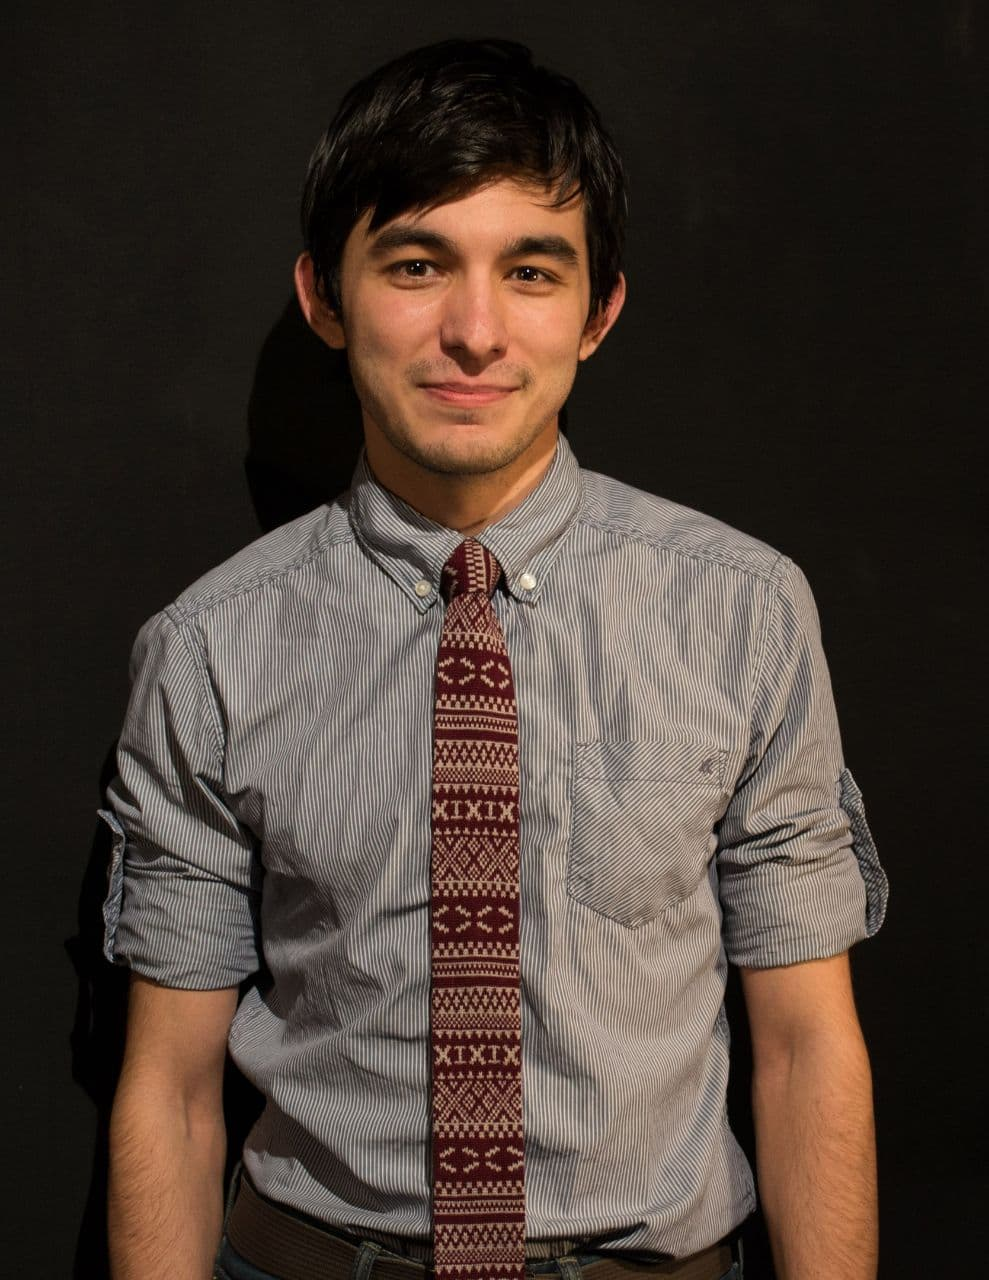
\includegraphics[width=\linewidth]{image}

%---------------------------------------------------------------------------------------
%	HEADER
%----------------------------------------------------------------------------------------
            \fcolorbox{white}{white}{\begin{minipage}[c][2.5cm][c]{1\mpwidth}
                                         \LARGE{\textbf{\textcolor{maincol}{Rival}}} \\[4pt]
                                         \LARGE{\textbf{\textcolor{maincol}{Abdrakhmanov}}} \\[4pt]
                                         \normalsize{ \textcolor{maincol}{.NET Developer} }
            \end{minipage}} \\

%---------------------------------------------------------------------------------------
%	CONTACTS
%----------------------------------------------------------------------------------------
            \cvsection{Contacts}

            \icontext{MapMarker}{16}{Saint Petersburg, Russia}{black}\\[2pt]
            \iconhref{Home}{16}{Blog}{https://rafaelldi.blog/}{black}\\[2pt]
            \iconhref{Github}{16}{GitHub}{https://github.com/rafaelldi}{black}\\[2pt]
            \iconhref{Twitter}{16}{Twitter}{https://twitter.com/rafaelldi}{black}\\[2pt]
            \iconhref{Linkedin}{16}{LinkedIn}{https://linkedin.com/in/rivalabdrakhmanov}{black}\\[2pt]

            \newpage
%---------------------------------------------------------------------------------------
%	SKILLS
%----------------------------------------------------------------------------------------
            \cvsection{Skills}

            \cvskill{.NET/C\#} {6+ yrs.} {1} \\[2pt]
            \cvskill{Web development} {4+ yrs.} {0.66} \\[2pt]
            \cvskill{Distributed systems} {3+ yrs.} {0.5} \\[2pt]
            \cvskill{Diagnostics} {1+ yrs.} {0.16} \\[2pt]
            \cvskill{Kotlin} {1+ yrs.} {0.16} \\[2pt]

%---------------------------------------------------------------------------------------
%	LANGUAGES
%----------------------------------------------------------------------------------------
            \cvsection{Languages}

            \cvskill{Russian} {Native} {1} \\[2pt]
            \cvskill{English} {B2} {0.8} \\[2pt]

%---------------------------------------------------------------------------------------
%	QR CODE
%----------------------------------------------------------------------------------------
            \vfill
            \cvqrcode{0.7}
        \end{leftcolumn}

        \begin{rightcolumn}
%---------------------------------------------------------------------------------------
%	PROFILE
%----------------------------------------------------------------------------------------
            \cvsection{About me}

            \vspace{4pt}

            \cvtext{
                Hi, my name is Rival, and I'm a .NET developer.

                During my career, I managed to work on different projects. Lately, I have dealt with distributed business applications.

                I like programming, so I often try some approaches and technologies and explore new areas in my free time. Recently, I've been fond of application diagnostics. I have a blog where I describe the results of my study. I try to be active in the community - I attend meetups, conferences, sometimes speak at them myself. Also, I'm working on my pet projects, such as \href{https://plugins.jetbrains.com/plugin/16426-tye}{Tye plugin for Rider}.

                I would be interested in working in a strong team on complex projects.
            }

%---------------------------------------------------------------------------------------
%	WORK EXPERIENCE
%----------------------------------------------------------------------------------------
            \vspace{10pt}
            \cvsection{Work experience}
            \vspace{4pt}

            \cvevent
            {07/2019 - today}
            {Software Developer}
            {Positive Technologies}
            {I'm working on various high load event-based projects on handling information security incidents.}
            {\cvlist{
                \item Projects: FinCERT, PT IPC, MaxPatrol 02
                \item Technologies and concepts: .NET, PostgreSQL, RabbitMQ, Kafka, Docker, DDD, CQRS, Event Sourcing, Microservices
            }}
            \vfill\null

            \cvevent
            {12/2017 - 07/2019}
            {Software Developer}
            {Radario LLC}
            {I was developing high load web application for event industry with microservices approach, creating high performance analytics and reporting service with ClickHouse as database, creating mobile application with Xamarin.Forms.}
            {}
            \vfill\null

            \cvevent
            {01/2017 - 12/2017}
            {Software Developer}
            {Splat}
            {I was creating desktop application for sport analytics with different metrics and coefficients of live match. }
            {}
            \vfill\null

            \cvevent
            {03/2016 - 01/2017}
            {Software Developer}
            {Promt}
            {I was creating system of machine based translation, working on statistical machine translation, building language models. By doing this I was working with statistical modeling, machine learning, natural language processing, computational linguistics.}
            {}
            \vfill\null

            \cvevent
            {12/2015 - 03/2016}
            {Testing Engineer}
            {NVision Group}
            {I was working as part of the emergency testing team, testing critical bugs from production. }
            {}
            \vfill\null

            \newpage
%---------------------------------------------------------------------------------------
%	EDUCATION
%----------------------------------------------------------------------------------------
            \cvsection{Education}

            \cvevent
            {2010 - 2015}
            {Mathematician, System Programmer}
            {Saint Petersburg State University}
            {Master's thesis: <<Monte Carlo method for integral equations in financial mathematics>>.}
            {}
            \vfill\null

%---------------------------------------------------------------------------------------
%	COURSES
%----------------------------------------------------------------------------------------
            \cvsection{Courses}

            \cvevent
            {04/2021}
            {\href{https://academy.dotnetos.org/certificates/sujhbeo6nl}{.NET Diagnostics Expert (EN)}}
            {Dotnetos Academy}
            {}
            {}
            \vfill\null

            \cvevent
            {05/2020}
            {\href{}{Advanced Distributed Systems Design using SOA \& DDD}}
            {Particular Software}
            {}
            {}
            \vfill\null

%---------------------------------------------------------------------------------------
%	TALKS
%----------------------------------------------------------------------------------------
            \cvsection{Talks}

            \cvevent
            {12/2020}
            {\href{https://youtu.be/TuKNdm4XBp4}{Patterns of distributed systems in the traditions of Russia’s northern indigenous and minority peoples}}
            {DOTNEXT 2020}
            {}
            {}
            \vfill\null

            \cvevent
            {10/2019}
            {\href{https://youtu.be/r16Zx591LJs}{HttpClient: common mistakes and ways to avoid them}}
            {SpbDotNet meetup}
            {}
            {}
            \vfill\null


% to create fake-space to ensure the whole height is used
            \vspace{25cm}

        \end{rightcolumn}
    \end{paracol}


\end{document}